\subsection{Time-walk corrections}
\label{sect:Time-walk}

\iffalse
{\it Note:
compare different techniques, including justification of NOT using laser calibration technique\\ $(http://www.jlab.org/Hall-B/notes/clas_notes93/note93-024.pdf)$\\
}
\fi

In order to optimize the time resolution, the time-walk caused by the height dependent timing variation based on Leading Edge Discriminator (LED) measurements has to be corrected. 
These time-walk corrections for the CLAS6 forward time-of-flight detector have been determined by using a laser-based calibration system~\cite{clastof}. This system consists of  four ultraviolet (UV) lasers. The UV light is delivered
to the center of each scintillator via a silica
optical fiber.  The TDC and ADC information
from the injected laser pulses can then be used to calibrate
the overall timing and pulse-height dependent time-walk. 

Due to the improved time resolution of the new CLAS12 time-of-flight panel 1b the previously used method is no longer sufficient and is replased by an in-situ calibration based on the accumulated data itself.
 The reasons for that are the following: a) In contrast to laser light that is delivered only to the center of
the scintillator, physical data are gathered along the whole bar length. The in-situ calibration facilitates a development of position-dependent time-walk corrections, thus improving the time resolution. b) The energy distribution of the particles and the shape of the analog signals that will be used for time-walk corrections will be by definition the same as in experiment, while the laser system injects monochromatic photon pulse with preselected amplitudes not corresponding to the experimental conditions.

During development and construction and before the installation into the CLAS12 detector all scintillation counters have been evaluated and checked using cosmic ray particles. The energy deposit of cosmic muons is relatively close to that of the particles  measured by CLAS12. Moreover, since cosmic muons are distributed homogenously along the scintillator, position-dependent time-walk corrections are applied. As mentioned  in Sec.~\ref{sec:six-bars} the typically used six-bars method demands that six counters are set up one above the other and that all PMT signals are coincide. 

After two days of running a sufficient amount of data was collected for each setup to carry out the analysis. The starting point of time-walk corrections procedure is ADC offsets substruction. Fig.~\ref{fig:offset} (left plot) shows ADC distribution zoomed in offset region. The offset peak position marked by red line was substracted from ADC values event by event. Shifted distribution is shown on the right plot of Fig.~\ref{fig:offset}. For further analysis all events that correspond to the offset peak were cut away.  


\begin{figure}[]
\begin{center}
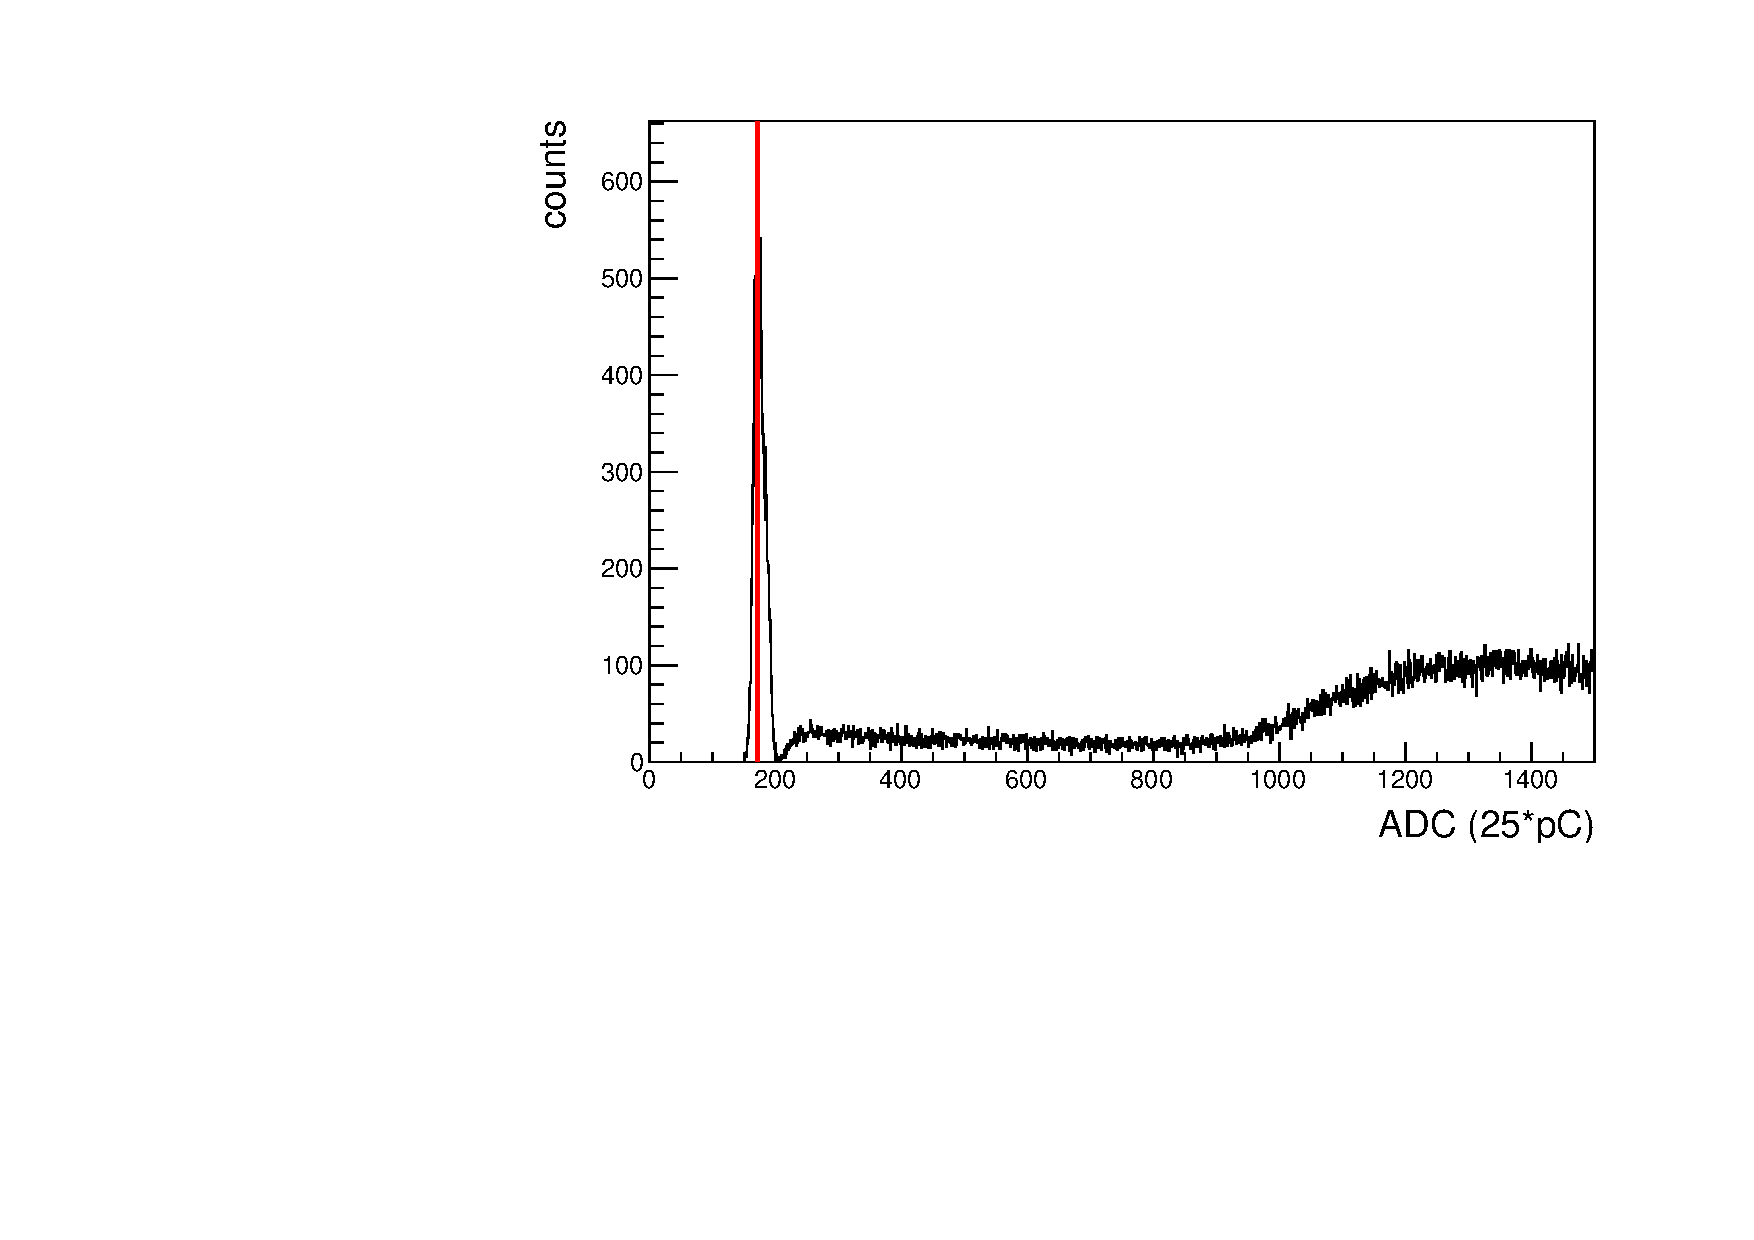
\includegraphics[width=3in]{gleb/fig_gleb_time_walk/offset.pdf}
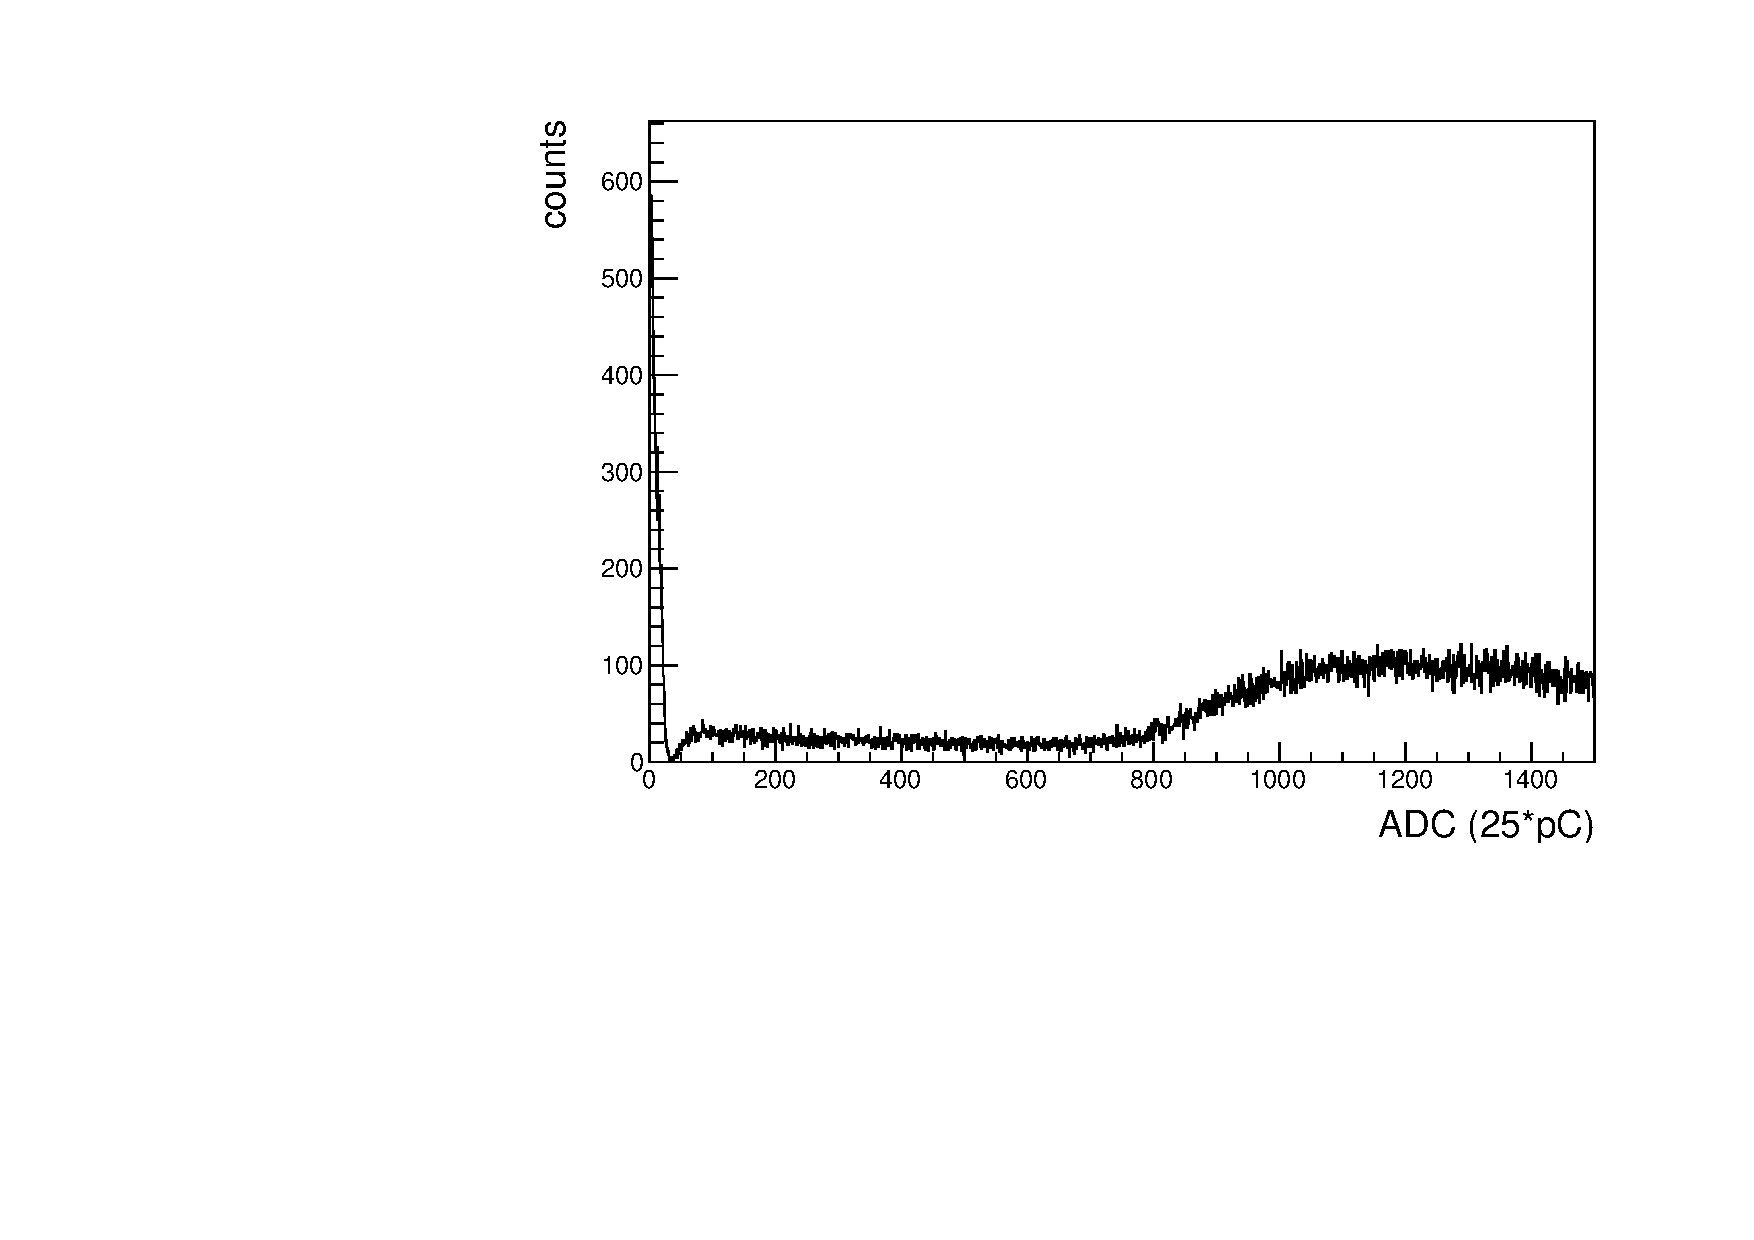
\includegraphics[width=3in]{gleb/fig_gleb_time_walk/offset_shifted.pdf}
\caption{ADC distribution zoomed in offset region before (left plot) and after (right plot) ADC offset substraction. Vertical red line on the left plot shows the position of the offset peak. \label{fig:offset}}
\end{center}
\end{figure}

The next step is vertical tracks selection that is not necessary for the method itself, but needed since position-dependent procedure is going to be applied. For that purpose the TDC difference between left and right PMTs for  bottom counter versus the same quantity for the top one (see Fig.~\ref{fig:vert_cut}) were plotted. These differences are divided over two since at that case they correspond to the bar length divided by effective speed of light. To determine the position of the red line (see Fig.~\ref{fig:vert_cut}) one dimentional distribution of the quantity $x - y$ was plotted (see Fig.~\ref{fig:diff_between_diff}), where $x = (tdc1-tdc2)/2$ and $y = (tdc11-tdc12)/2$. These quantities correspond to the $x$ and $y$ axes of the two dimentional plot Fig.~\ref{fig:vert_cut}. This one dimentional distribution was fitted by gaussian to determine the mean value $M$ (see Fig.~\ref{fig:diff_between_diff}). The line with equation $y = x + M$ is drawn by red on Fig.~\ref{fig:vert_cut}.For analysis the whole bar length was divided into the bins approximatly 3 cm width each. The range over x-axis that correspond to the scintillator length was divided into the same number of bins. 
Bin size over y-axis was determined by intersections of boundaries of the bin over x-axis with red line.
Events within rectangular area (shown in white on Fig.~\ref{fig:vert_cut}) were selected for further analysis.  
All steps described below correspond to one particular bin.

\begin{figure}[]
\begin{center}
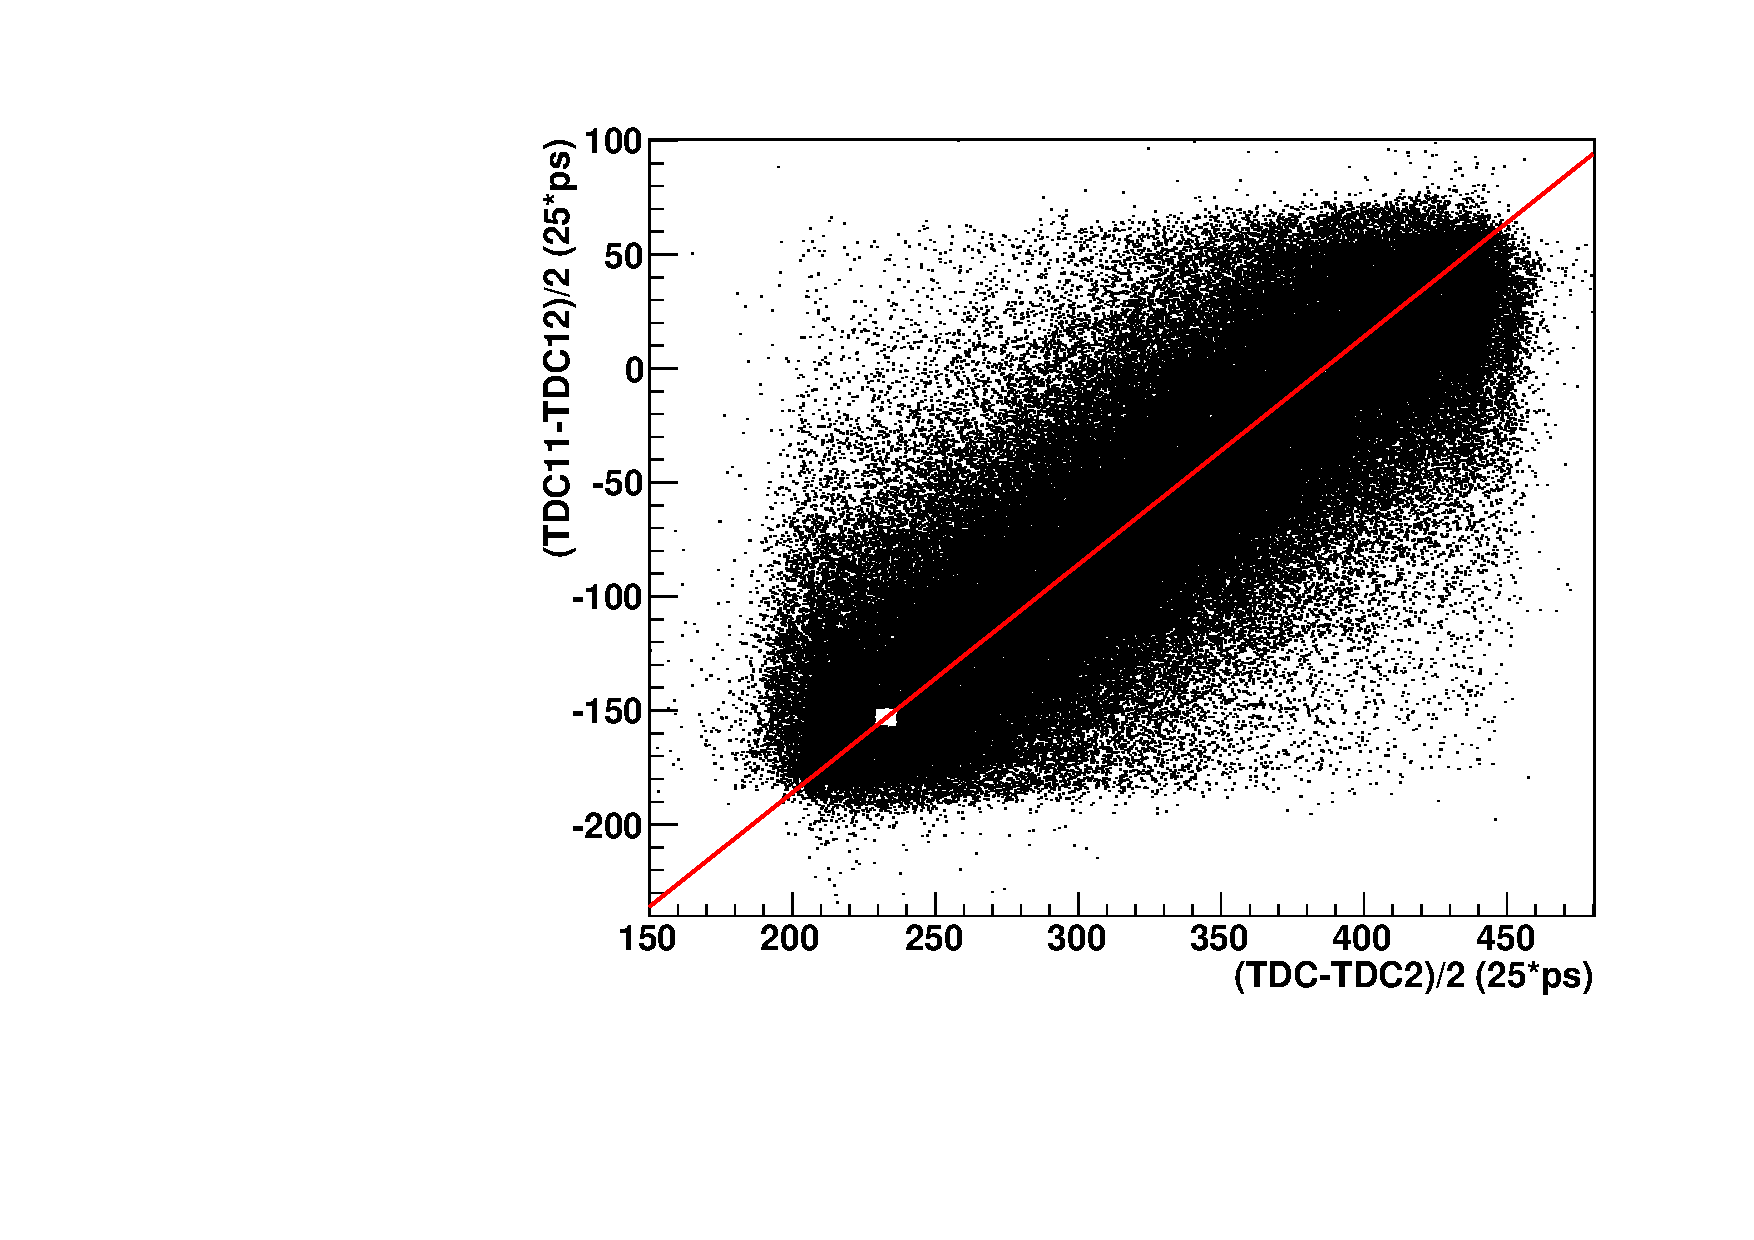
\includegraphics[width=3in]{gleb/fig_gleb_time_walk/vert_cut.pdf}
\caption{TDC difference between left and right PMTs for  bottom counter versus the same quantity for the top one. Plot corresponds to the bars 81cm long from the set number eleven. The position of red line is determined by fitting of distribution shown on Fig.~\ref{fig:diff_between_diff}. Rectangular area shown in white is one of the bins that was used for time-walk parameters determination. \label{fig:vert_cut}}
\end{center}
\end{figure}

\begin{figure}[]
\begin{center}
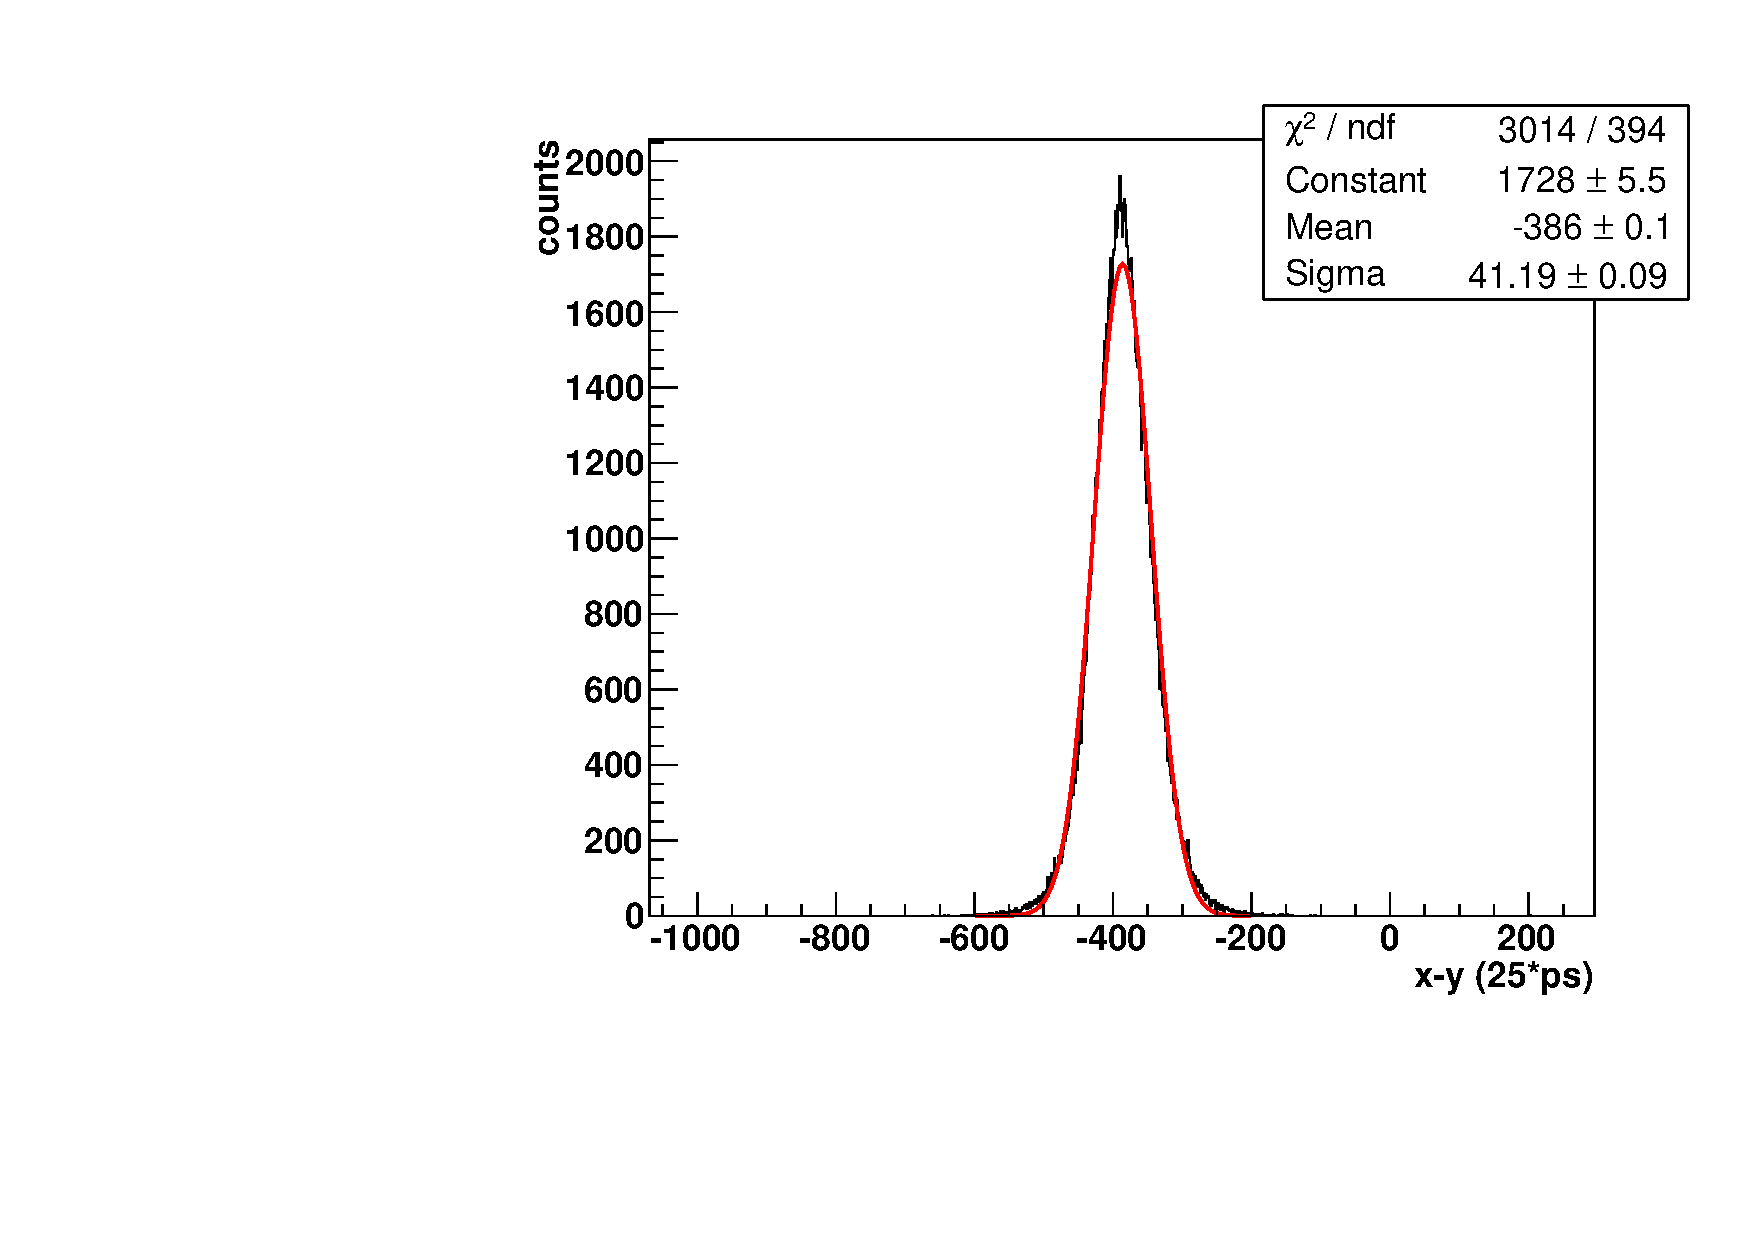
\includegraphics[width=3in]{gleb/fig_gleb_time_walk/vert_cut_fit.pdf}
\caption{$x-y$ distribution, where $x = (TDC1-TDC2)/2$ and $y = (TDC11-TDC12)/2$. Mean value of gaussian fit determine position of red line on Fig.~\ref{fig:vert_cut}. \label{fig:diff_between_diff}}
\end{center}
\end{figure}
Time-walk is an instrumental pulse height dependent shift in the measured time using a leading edge discriminator~\cite{Leo:1987kd}. This time difference is due to the finite rise time of the analog pulse reaching the threshold relative to a reference time. This effect can be minimized in hardware by using constant-fraction discriminators, or by making software corrections to the times using leading-edge discriminators. Since leading-edge discriminator is used one-parameter ($\lambda_i$) time-walk correction is applied to each PMT, where $i$ corresponds to the PMT number.  
In the experemental setup reference time is given by PMT number five, which is attached to the left side of the bar number three. This PMT determines the relative timing of all the other signals.
Accordingly, a single relative time depends on two parameters ($\lambda_i$ and $\lambda_{ref}$) as in Eq.~\ref{eq:t_corr}.
In equation~\ref{eq:t_corr} the second term in each parenthesis is introduced in order to take into account signal rise time.

\begin{equation}
t_{corrected} = \left( TDC_i - \frac{\lambda_i}{\sqrt{ADC_i}} \right) - \left( TDC_{ref} - \frac{\lambda_{ref}}{\sqrt{ADC_{ref}}} \right)
\label{eq:t_corr}
\end{equation}

For each ionizing particle
path $t_{corrected}$ is ideally fixed, so the spreading $\sigma$ of the Gauss fit of the $t_{corrected}$ distribution 
 on a specifed path must be minimized with the two-parameter correction function. For that purposes  each parameter $\lambda$  is varied within the range from -2 to 6, where the spreading of the $t_{corrected}$ distributions is minimal, and plotted as a color code on two dimensionals histograms (see Fig.~\ref{fig:tw_param}). On Fig.~\ref{fig:tw_param} $\lambda_5$ versus $\lambda_i$ is plotted for each PMT except PMT number six since signals from the PMTs five and six are correlated, because they are connected to the same bar. That is why to determine $\lambda_6$  $\lambda_7$ versus $\lambda_6$ is plotted. 






\begin{figure}[]
\begin{center}
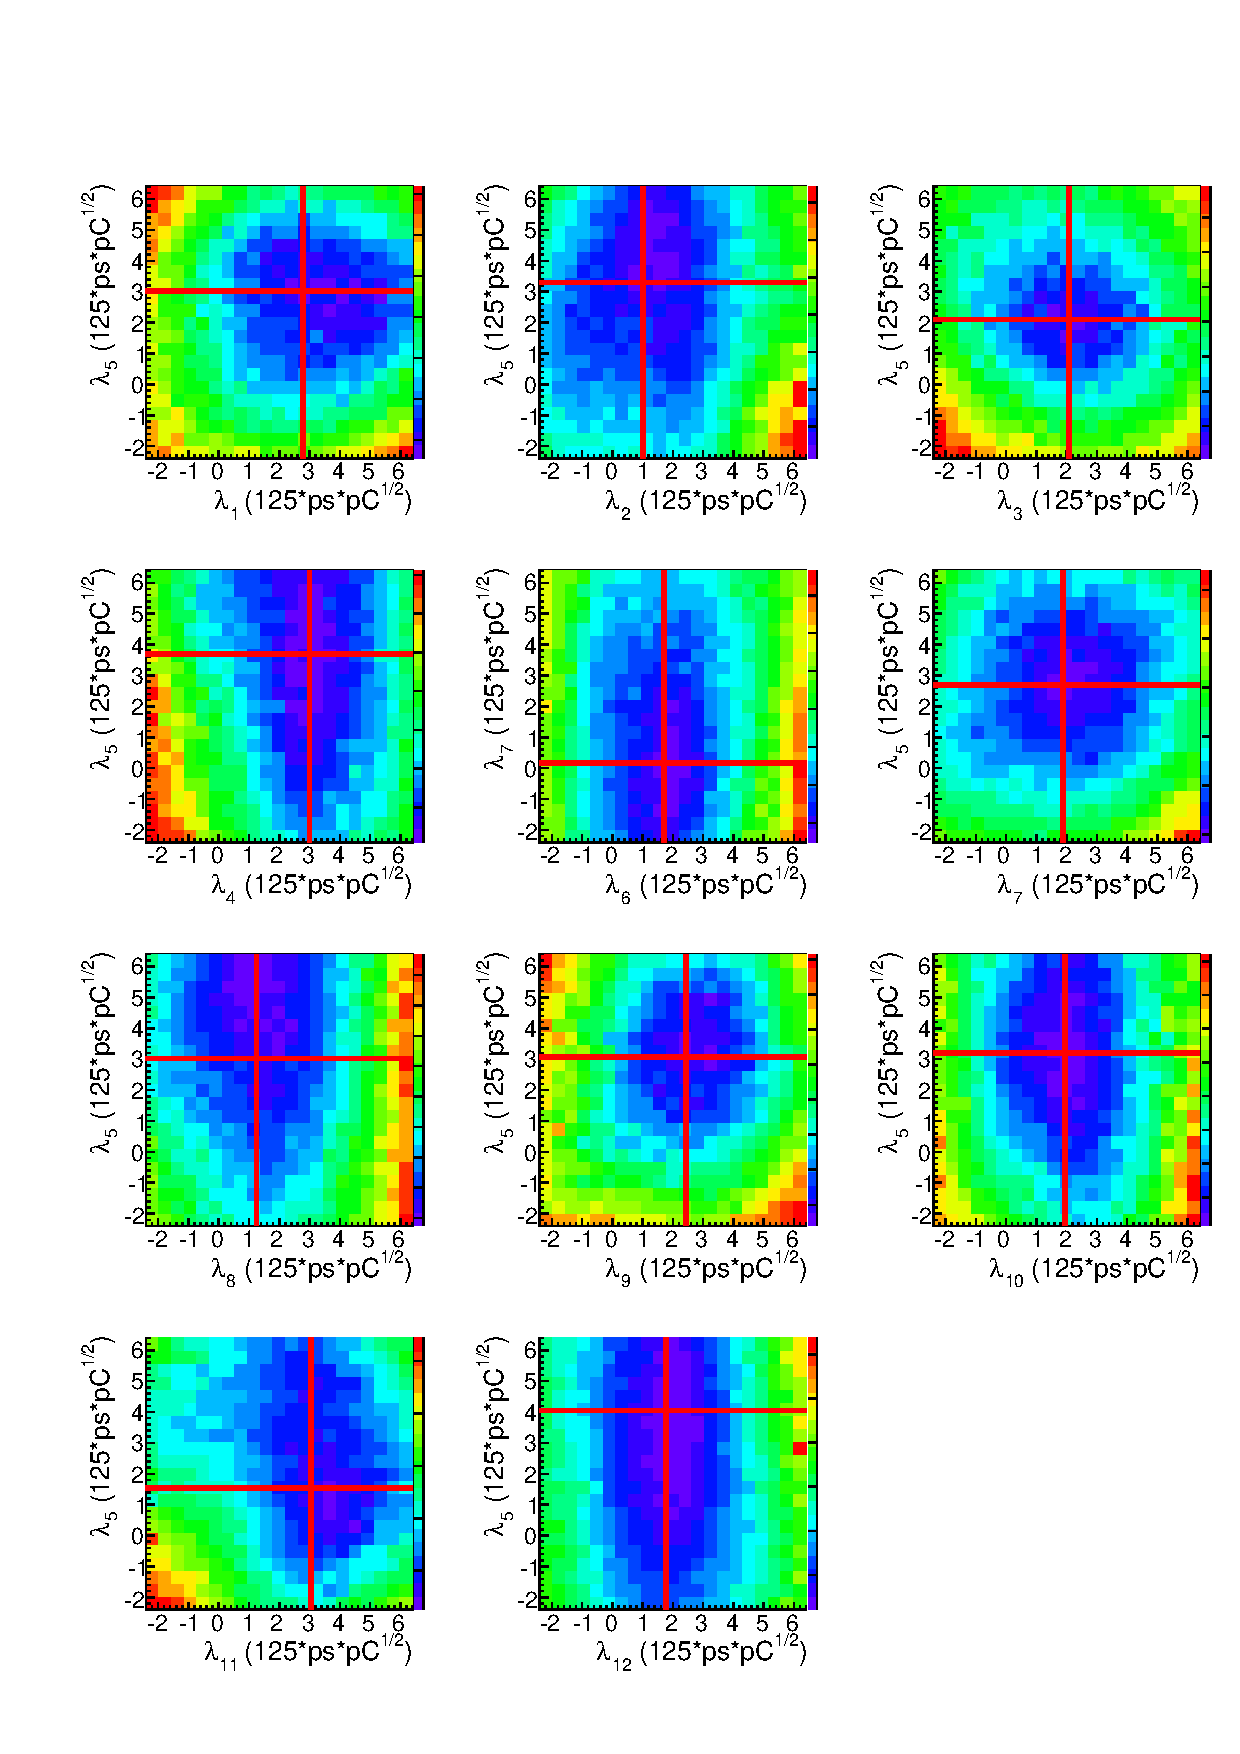
\includegraphics[width=5in]{gleb/fig_gleb_time_walk/tw_param.pdf}
\caption{Two dimensional distributions used to determine time-walk parameters. Coordinate axes correspond to time-walk parameters $\lambda_{i}$ varied from -2 to 6 each. Color code represents spreading of the $t_{corrected}$ distributions (see Eq.~\ref{eq:t_corr}). \label{fig:tw_param}}
\end{center}
\end{figure}

In order to determine the position of the minimum each distribution from Fig.~\ref{fig:tw_param} is fitted by parabolic function. The intersections of red lines show positions of obtained minima. The $x$-coordinate of each minima gives value of $\lambda$ parameters for all PMTs, except PMT five. Since almost all distributions have $\lambda_5$ as $y$-axis, $\lambda_5$ is determined as average value of $y$-coordinates of the minuma for these distributions.


\begin{figure}[]
\begin{center}
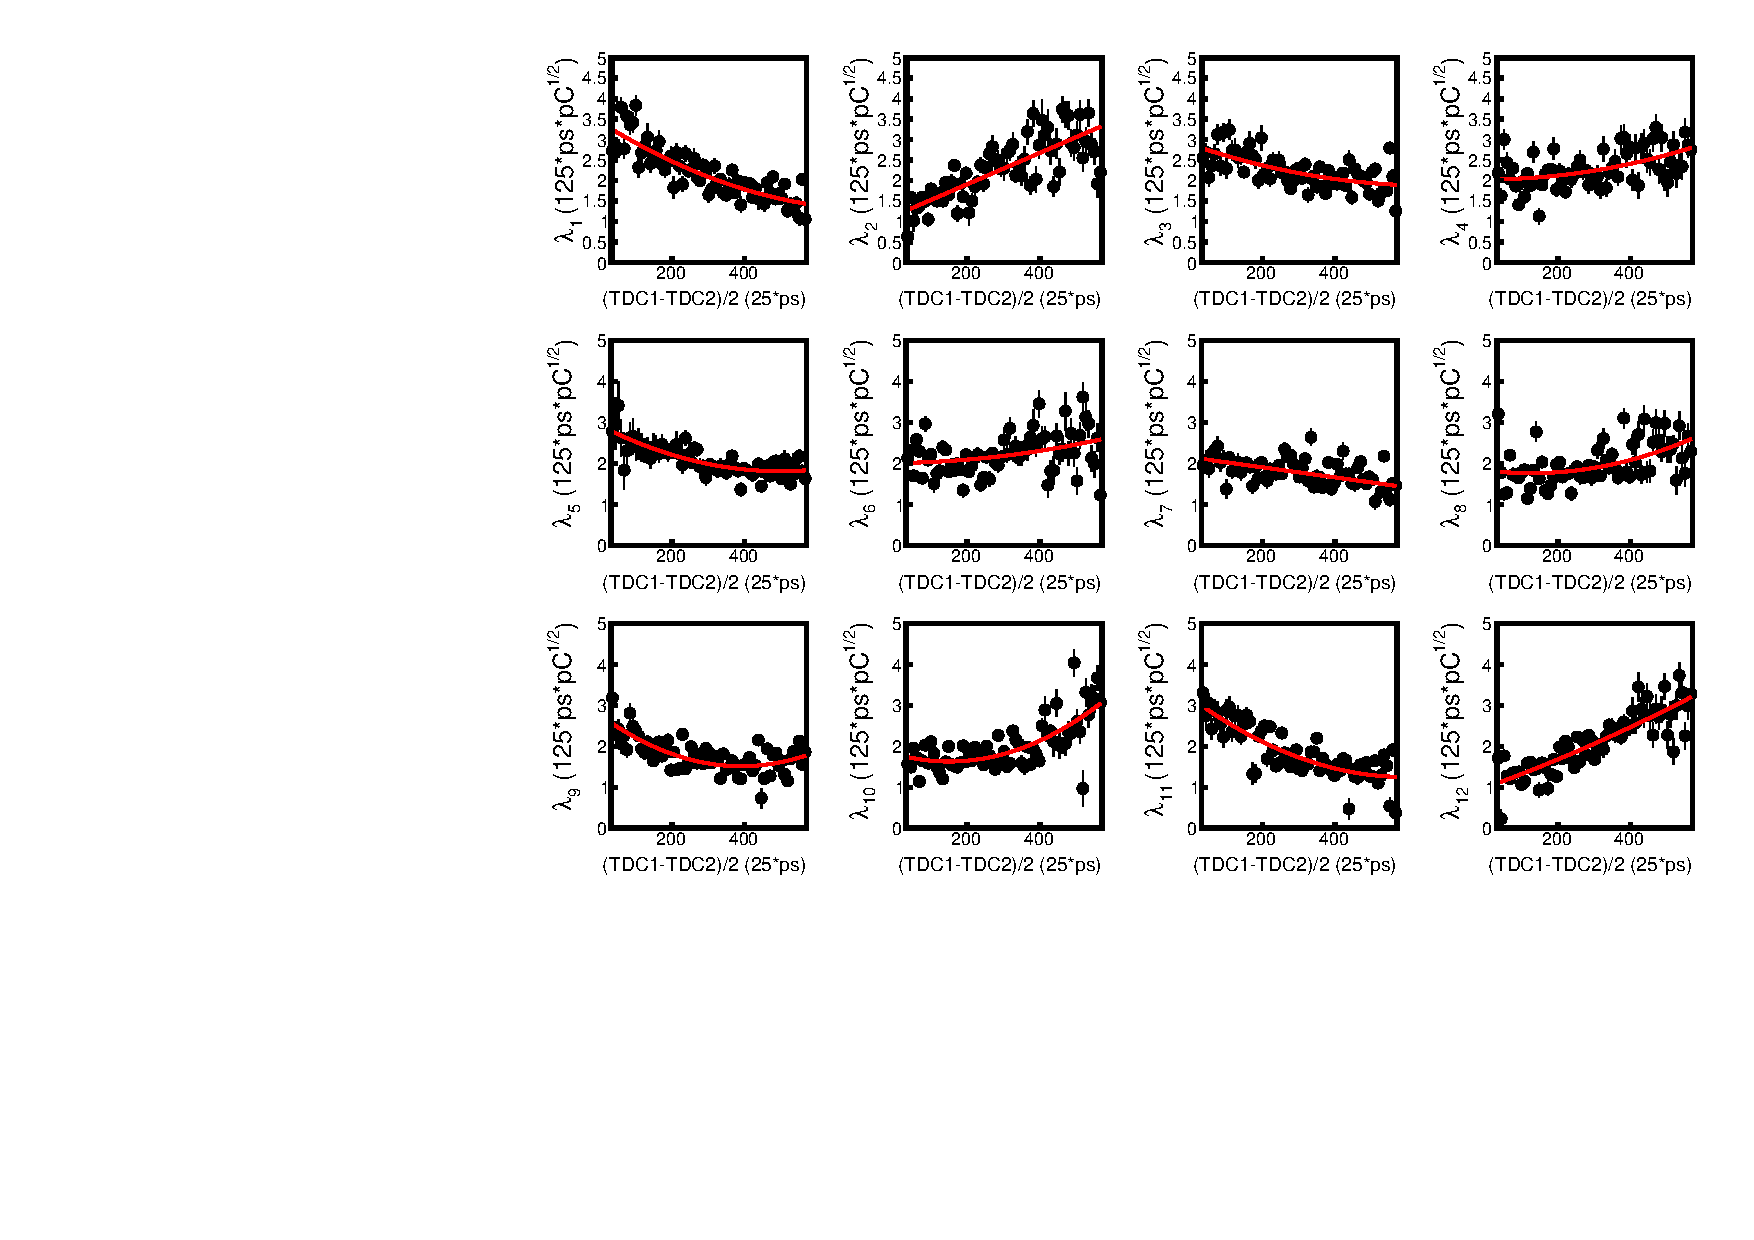
\includegraphics[width=5in]{gleb/fig_gleb_time_walk/tw_params_1d.pdf}
\caption{Time-walk parameters as function of the half of the TDC differences for the bars 200 cm long from the set number 30. Curves represent second order polynomial fit. \label{fig:tw_param_1d}}
\end{center}
\end{figure}

The procedure described above is applied for each bin from Fig.~\ref{fig:vert_cut}. On Fig.~\ref{fig:tw_param_1d}  all extracted $\lambda$ parameters are plotted as a function of TDC differences divided by two that correspond to the length of the scintillator bar. $\lambda$-distribution for each PMT is fitted by second order polynomial. Finally for calculations of time-walk corrected times $\lambda$-parameters as smooth function of bar length is used.
 




